\documentclass[12pt,a4paper]{article}

\usepackage{amsmath,amssymb,amsfonts,amsthm}
\usepackage{mathtools}
\usepackage{fullpage,setspace}
\usepackage{caption}
\usepackage{subcaption}
\usepackage{enumitem}
\usepackage{float}
\usepackage{framed}
\usepackage{fancyhdr}
\usepackage[colorinlistoftodos]{todonotes}
\usepackage[english]{babel}
\usepackage[utf8]{inputenc}
\usepackage{algorithm}
\usepackage{algpseudocode}
\usepackage{verbatim}
\usepackage{algorithmicx}
\usepackage{mathrsfs}
\usepackage{booktabs}
\usepackage{titling}
%\usepackage{array}
\usepackage{multicol}
\usepackage{lmodern}
\usepackage{float}
\usepackage{graphicx}
\graphicspath{images}
\usepackage{indentfirst} % indent first paragraph
\usepackage{hyperref} % table of content links
\hypersetup{
    colorlinks=true,
    allcolors=black
}

\DeclareMathOperator{\sign}{sign}

\DeclarePairedDelimiter\abs{\lvert}{\rvert}%
\DeclarePairedDelimiter\norm{\lVert}{\rVert}%

% Swap the definition of \abs* and \norm*, so that \abs
% and \norm resizes the size of the brackets, and the 
% starred version does not.
\makeatletter
\let\oldabs\abs
\def\abs{\@ifstar{\oldabs}{\oldabs*}}
%
\let\oldnorm\norm
\def\norm{\@ifstar{\oldnorm}{\oldnorm*}}
\makeatother

\newcommand*{\Value}{\frac{1}{2}x^2}%
\usepackage[top=.5in, bottom=1in, left=.5in, right=.5in]{geometry}
%\newcommand{\addpic}[1]{\includegraphics[width=14em]{#1}}
%\newcolumntype{C}{>{\centering\arraybackslash}m{14em}}

\title{APMA 1360: Homework Assignment \#2}
\pretitle{\begin{center}\fontsize{20bp}{18bp}\selectfont}
\posttitle{\par\end{center}}
\author{Eli Berkowitz}
\predate{}
\date{Feb 15 2017}
\postdate{}

\begin{document}

\maketitle

\section{Question 1}

Let $f(u) = \dot{u} = 1 + \mu u + u^2$.
\begin{itemize}
    \item Equilibria:
    \begin{align}
    f(u) = 0 &= 1 + \mu u + u^2 \\
             \implies u &= \frac{-\mu \pm \sqrt{\mu^2 - 4}}{2} \\
             u_1 &= \frac{1}{2}{\left( -\mu + \sqrt{\mu^2 - 4}\right)} \\
             u_2 &= -\frac{1}{2}{\left(\mu + \sqrt{\mu^2 - 4}\right)}
    \end{align}

    Depending on $\mu$, the equilibra are:

    $$\begin{cases}
        \{\} & |\mu| < 2 \\
        \{1, -1\} & |\mu| = 2 \\
        \left\{\frac{1}{2}{\left( -\mu + \sqrt{\mu^2 - 4}\right)},
        -\frac{1}{2}{\left(\mu + \sqrt{\mu^2 - 4}\right)}\right\} & |\mu| > 2
    \end{cases}
        $$
    \item Equilibria Stability
        $$f'(u) = \mu + 2u$$
    \begin{itemize}
        \item $u_1$ $$f'(u_1) = \mu + 2{\left(\frac{1}{2}{\left( -\mu + \sqrt{\mu^2 - 4}\right)}\right)} = \sqrt{\mu^2 - 4}$$
        \item $u_2$ $$f'(u_2) = \mu + 2{\left(-\frac{1}{2}{\left(\mu + \sqrt{\mu^2 - 4}\right)}\right)} = -\sqrt{\mu^2 - 4}$$
    \end{itemize}
    \textbf{$u_1$ and $u_2$ are always semistable.}
    \item Bifurcation Diagram
    \begin{figure}[H]
        \centering
        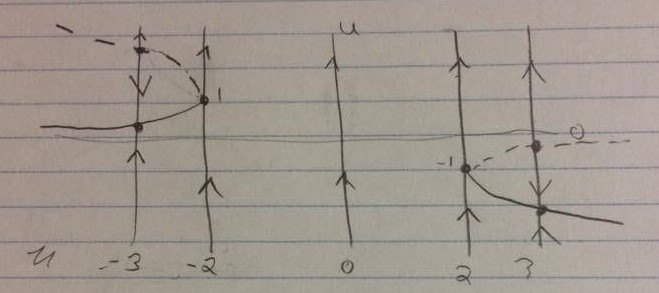
\includegraphics[width=0.7\textwidth]{q1-bifurcation}
    \end{figure}

\end{itemize}
\section{Question 2}

Let $\dot{u} = f(u, \mu) = \sin{\mu} + (1 + \mu)\cdot u \sin{u} - u^3 e^u$.

To be a saddle node bifurcation, $f(u, \mu)$ must satisfy these conditions:

\begin{itemize}
    \item $f_{uu}(u_0, \mu_0) \neq 0$
    \begin{align}
    f_u &= (1 + \mu)(u\cos{u} + \sin{u}) - (3u^2 e^u + u^3 e^u) \\
    f_{uu} &= (1 + \mu)(-u\sin{u}+2\cos{u}) - (6u e^u + 6u^2 e^u + u^3 e^u) \\
    f_{uu}(0, 0) &= 2 \neq 0
    \end{align}
    \item $f_\mu(u_0, \mu_0) \neq 0$
    \begin{align}
        f_\mu &= \cos{\mu} + u\sin{u} \\
        f_\mu(0, 0) &= 1 \neq 0
    \end{align}
\end{itemize}

Since $f(u, \mu)$ satisfies both conditions, it is a saddle node bifurcation.

Now, using the result from class:

$$\mu = g(u) = u_0 - \frac{f_{uu}(u_0,\mu_0)}{2f_\mu(u_0, \mu_0)}\cdot (u - u_0)^2 + O(\abs{u - u_0}^3) = 0 - \frac{2}{2\cdot1}\cdot u^2 + O(\abs{u}^3) = -u^2 + O(u^3)$$

This implies that the bifurcation diagram will have a parabola opening leftward, $\mu \approx -u^2$. To determine the stability of the equilibria, using the other result from class:

$$\text{Stability if }\sign{f_{uu}(u_0, \mu_0)(u-u_0)} \text{ is } \begin{cases}\text{Stable}&+\\\text{Unstable}&-\end{cases}$$

$$f_{uu}(u_0, \mu_0)(u-u_0) = 2u$$, so where $u > 0$, the equilibria are stable, and where $u < 0$, the equilibra are unstable.

All of this information yields this bifurcation diagram:

\begin{figure}[H]
    \centering
    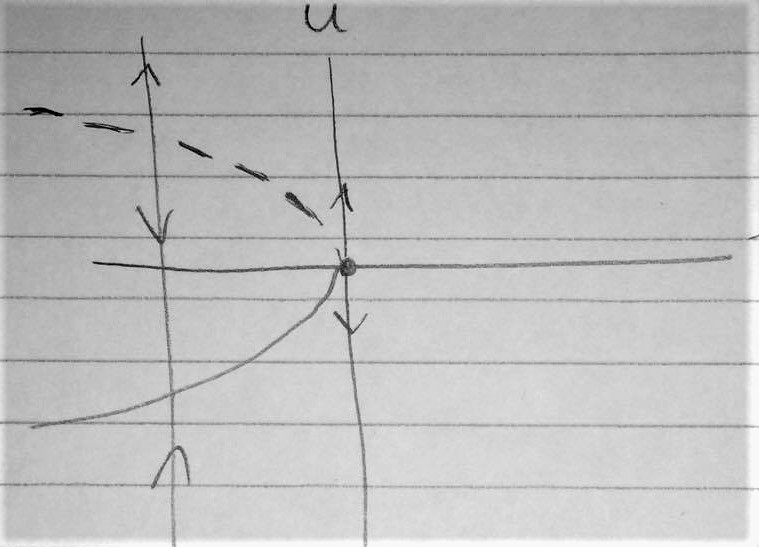
\includegraphics[width=0.7\textwidth]{q2-bifurcation}
\end{figure}

\section{Question 3}

\begin{figure}[H]
\centering
\begin{subfigure}{.3\textwidth}
    \centering
    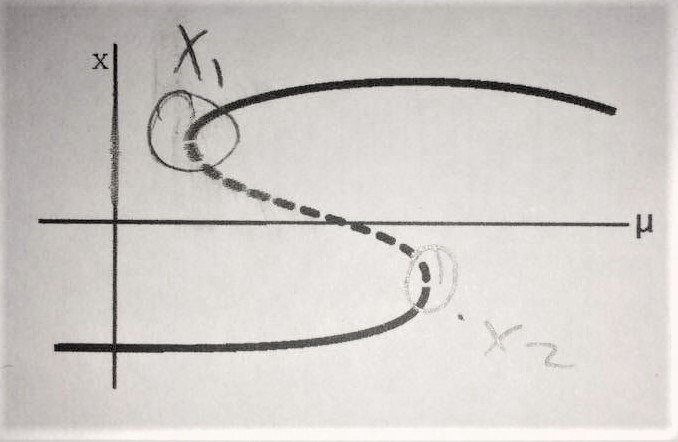
\includegraphics[width=.8\linewidth]{q3-a}
    \caption{$x_1$ and $x_2$ are saddle-node bifurcation points}
\end{subfigure}
\begin{subfigure}{.3\textwidth}
    \centering
    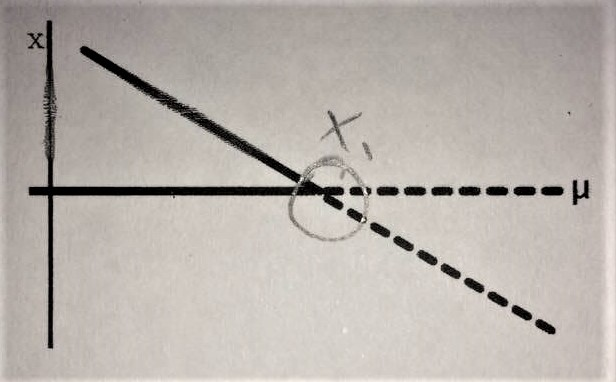
\includegraphics[width=.8\linewidth]{q3-b}
    \caption{$x_1$ is a transcritical bifurcation point.}
\end{subfigure}
\begin{subfigure}{.3\textwidth}
    \centering
    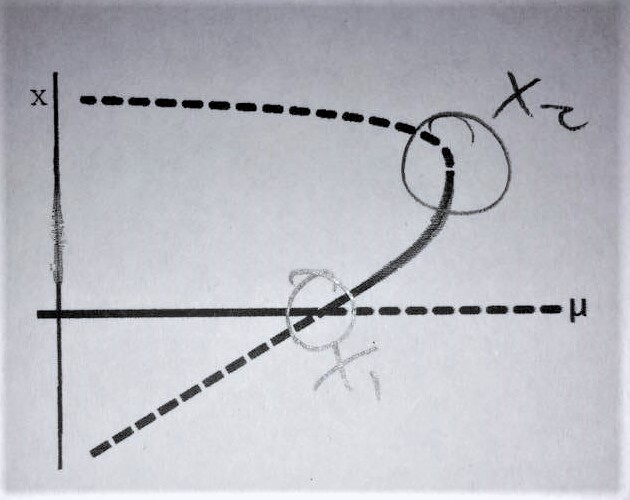
\includegraphics[width=.8\linewidth]{q3-c}
    \caption{$x_1$ is a transritical bifurcation. $x_2$ is a turning point bifurcation.}
\end{subfigure}
\end{figure}



\section{Question 4}

Let $f(u) = \frac{du}{dt} = u\cdot g(u, \mu)$.

\begin{enumerate}[label=(\roman*)]
\item
Setting $f(u) = 0$ reveals all equilibria:

$$f(u) = 0 = u\cdot g(u, \mu) \implies u = 0 \text{ or } g(u, \mu) = 0$$
\item 
\end{enumerate}
\end{document}
